\documentclass[a4paper, titlepage, 12pt, openright, twoside]{book}

\usepackage[T1]{fontenc}
\usepackage[italian]{babel}
\usepackage{frontespizio}
\usepackage{booktabs}
\usepackage{graphicx}
\usepackage{amsmath}
\usepackage{stmaryrd}
\usepackage{cite}
\usepackage[utf8]{inputenc}
\usepackage{lmodern}
\usepackage{algorithm}
\usepackage{algpseudocode}

\graphicspath{ {./img/} }
\floatname{algorithm}{Algoritmo}

\begin{document}

\begin{frontespizio}
\Universita{Verona}
\Dipartimento{Informatica}
\Corso[Laurea]{Informatica}
\Titoletto{Tesi di laurea}
\Titolo{Architetture per la gestione di ordini in locali di ristorazione}
\NCandidato{Studente}
\Candidato[436988]{VACCARI NICOLAS}
\Annoaccademico{2022-2023}
\end{frontespizio}

\tableofcontents

\chapter{Introduzione}\label{chap:introduzione}

\section{Prefazione}

Questo documento ha come obbiettivi:
\begin{itemize}
	\item dare al lettore una panoramica sullo stato della ristorazione e della sua importanza al momento della scrittura
	\item quali possono essere le esigenze degli enti e gestori che mettono a disposizione un servizio di ristorazione aziendale collettivo descrivendo un caso d'uso
	\item quali soluzioni digitali è possibile adottare al fine di soddisfare i requisiti e quali criticità sussistono nella realizzazione di tali soluzioni
\end{itemize}

Il documento non ha come scopo quello di illustrare le procedure burocratiche, economiche e operative che riguardano il mondo della ristorazione o le aziende coinvolte.

\section{Panoramica sul mercato della ristorazione}

A dicembre 2022 negli archivi delle Camere di Commercio italiane risultano attive 335.817 
imprese appartenenti al codice di attività 56.0 con il quale vengono classificati i servizi di ristorazione.
Un numero che non stupisce sia per un fattore culturale, sia perché i pubblici esercizi di questo tipo sono
una realtà ampiamente diffusa in ogni regione e che non ha eguali con nessun'altra tipologia di servizio rivolta al pubblico presente in Italia.
\newline
Nonostante negli ultimi 4 anni il settore abbia subito delle forti perdite economiche dovute principalmente alla pandemia COVID-19,
all'inflazione e alla diffusione dell'ideologia "Stay at home" con annesso food delivery, 
il 2022 ha dimostrato che il mercato è in fase di stabilizzazione e ripresa, con valore stimato di circa 82 miliardi,
avvicinandosi così al valore pre-pandemia del 2019 pari a 85.5 miliardi. \cite{rristorazione}
\newline
Questo settore, prevalentemente composto da manodopera umana e con un carico importante di legislazioni da rispettare, ha da sempre lasciato poco spazio all’introduzione della tecnologia, sia per una questione di convenienza economica, sia per una questione pratica. E’ infatti una sfida molto impegnativa sostituire un operatore di cucina o un cuoco, con strumenti tecnologici. Negli ultimi anni la produzione di macchinari (forni e attrezzature varie) sempre più connessi tra di loro ha reso possibile modalità di lavoro più efficienti ed efficaci, mentre i magazzini a gestione sempre più automatizzata e digitalizzata contribuiscono all'efficienza e alla sicurezza dello stoccaggio delle derrate alimentari.
\newline
Fortunatamente per il settore IT, grazie al cambiamento dello stile di vita della persona media influenzato dai fattori citati precedentemente,
i ristoratori (specialmente i ristoratori collettivi) sono sempre più alla ricerca di nuove soluzioni per attrarre nuovi clienti
e generare più vendite utilizzando gli stessi locali, aprendo così nuove possibilità di sviluppo per le aziende di software e di conseguenza nuove sfide tecnologiche da risolvere.

\section{Tipologie di ristorazione}

Il mondo della ristorazione si divide principalmente in due categorie:
\begin{itemize}
	\item \textbf{Ristorazione commerciale}: si rivolge direttamente al consumatore finale, con una clientela di tipo occasionale
											 (sono i clienti stessi che decidono di recarsi in quella specifica ubicazione) e nella maggior parte dei casi
											 propone alimenti che sono preparati e consumati nello stesso luogo. Confrontandola con la ristorazione collettiva,
											 il costo medio dei pasti è maggiore, ed il numero di individui che è possibile ospitare contemporaneamente è solitamente inferiore.
											 In questa categoria rientrano:
											 \begin{itemize}
											 	\item \textbf{Ristorazione tradizionale}: la più comune e conosciuta, include trattorie, pizzerie, bistrot, ...
											 	\item \textbf{Ristorazione agrituristica}: locali interni ad aziende agricole che offrono pietanze preparate con le proprie materie prime
											 	\item \textbf{Ristorazione alberghiera}: svolta all'interno di strutture alberghiere a completamento dell'offerta dei propri servizi
											 	\item \textbf{Ristorazione veloce}: quella in più rapida espansione, include tutte le attività 
											 										come fastfood, snackbar, tavole calde, ...
											 \end{itemize}
	\item \textbf{Ristorazione collettiva}: si occupa della preparazione e consegna di pasti su larga scala, con alimenti preparati in cucine industriali dedicate e
											successivamente distribuiti a cucine più piccole collocate all'interno dei refettori che hanno il compito di rigenerare l'alimento
											e consegnarlo al consumatore finale. I clienti di questo servizio sono tipicamente i fruitori dell'ambiente in cui si trova il locale
											(ad esempio i dipendenti di una azienda), diventando quindi clienti abituali con una scelta che deriva principalmente 
											dalla necessità di dover consumare almeno un pasto durante il loro periodo di permanenza nell'ubicazione. 
											I costi di produzione sono un elemento fondamentale che l'azienda di ristorazione cerca spesso di contenere al minimo.
											Il costo del pasto (o una parte di esso) può essere a carico dell'ente che mette a disposizione il servizio (es: azienda o università)
											configurandolo come un welfare per il dipendente. La modalità operativa cambia a seconda della tipologia di collettività trattata.
											Il servizio può essere erogato sotto forma di pasti venduti in una linea self-service, o serviti a degenti di un ospedale o di una
											casa di riposo, oppure ancora serviti nei refettori scolastici ad alunni e docenti.
											Le tipologie che identificano la ristorazione collettiva sono:
											\begin{itemize}
												\item \textbf{Ristorazione aziendale}: si trova all'interno di imprese di medie o grandi dimensioni ed è dedicata alla preparazione
																						del pranzo o cena per i dipendenti
												\item \textbf{Ristorazione scolastica}: dedicata alla preparazione di pasti per studenti e dipendenti di scuole e università
												\item \textbf{Ristorazione socio-sanitaria}: dedicata alla preparazione di pasti all'interno di ospedali, cliniche e case di riposo
												\item \textbf{Ristorazione assistenziale}: dedicata alla preparazione di pasti da distribuire al domicilio di persone 
																							non autosufficienti
												\item \textbf{Ristorazione comunitaria}: presente all'interno di caserme, istituti religiosi e carceri penitenziari
											\end{itemize}
\end{itemize}

\section{Il peso della ristorazione collettiva}

La ristorazione collettiva nasce con l'obbiettivo di colmare l'esigenza di tutti quegli individui
che hanno la necessità di consumare almeno un pasto fuori casa, solitamente per un fattore di tempo a disposizione.
Ad oggi possiamo considerare la ristorazione collettiva non più come "un plus" disponibile a pochi, ma una necessità di una società in continua evoluzione.
Fornendo un esempio, nel settore IT possiamo notare come le 5 aziende FAANG offrano un servizio di ristorazione di alta qualità aperto 14 ore al giorno ai propri collaboratori
e di come questo servizio venga valorizzato da loro stessi come un punto di forza fondamentale per l'azienda stessa.
\newline
Uscendo dal mondo delle migliori aziende di software, troviamo comunque sempre più casi dove gli enti puntano ad offrire come benefit un servizio mensa di media-alta qualità,
sia ai propri dipendenti che ai propri ospiti.
\newline
Ma quanto è effettivamente importante il servizio di ristorazione?
\newline
Un esempio illuminante per riflettere sulle dinamiche aziendali è rappresentato da Google. Nel tentativo di incoraggiare i propri dipendenti a ritornare in ufficio e lasciare il lavoro da casa, l'azienda ha introdotto un'interessante iniziativa. Oltre a fornire gratuitamente pasti per l'intera giornata lavorativa, Google offre anche un servizio di consulenza nutrizionale personalizzata svolto da un team specializzato. Questa iniziativa, inserita nel welfare aziendale, mira a promouovere uno stile di vita sano e a migliorare il benessere dei dipendenti.
In aggiunta a questo esempio, vale la pena considerare uno studio della Cornell University \cite{cornell}, che evidenzia diversi aspetti significativi in merito. L'articolo mette in luce che le strategie aziendali orientate al benessere dei dipendenti, come la fornitura di pasti e servizi nutrizionali, siano elementi importanti per la creazione di un ambiente di lavorativo sano e motivante. Un'attenzione particolare alla salute e al benessere può influenzare positivamente la produttività e la soddisfazione dei dipendenti, contribuendo allo sviluppo di una cultura aziendale positiva e orientata al supporto reciproco. Questi esempi evidenziano la crescente importanza che molte aziende attribuiscono alla salute e al benessere dei loro dipendenti, riconoscendo il valore di tali iniziative e come queste possano incidere positivamente sulla qualità del lavoro e sulla coesione aziendale.

\chapter{Caso d'uso: Refettorio aziendale}\label{chap:caso}

\section{Requisiti di ente e gestore}

Requisiti dell'azienda ente:
\begin{itemize}
	\item Possibilità di prenotare in anticipo il pasto entro 12 ore prima dall'inizio del turno in mensa
	\item Possibilità di ordinare in loco il pasto per gli utenti che non hanno prenotato
	\item Garantire che gli ordini effettuati vengano messi a disposizione rispettando l'ordine d'ingresso in coda al refettorio da parte del singolo utente
\end{itemize}

Requisti dell'azienda gestore:
\begin{itemize}
	\item Tenere traccia di tutti gli individui che usufruiscono della mensa, al fine di effettuare la rendicontazione e monitorare scorte e consumi
	\item Menù fisso con costo prestabilito e una combinazione composta da un primo piatto, un secondo piatto e un contorno
	\item Regolamentare gli orari entro il quale è possibile prenotare il pasto
	\item Regolamentare gli orari in cui il servizio mensa è attivo e gli orari di accesso al refettorio
	\item Due addetti alla linea self, uno per la gestione dei primi piatti e uno per la gestione dei secondi piatti e dei contorni
\end{itemize}

\section{Analisi dei requisiti}

Analizzando i requisiti di ente e gestore possiamo stilare i seguenti punti:
\begin{itemize}
	\item E' necessario introdurre un sistema centrale per il salvataggio dei menù, il salvataggio degli ordini in loco e delle prenotazioni,
		  l'elaborazione dei pagamenti, l'invio di email di conferma per le prenotazioni, regolazione degli orari di servizio, l'anagrafica degli utenti finali, l'anagrafica degli
		  utenti operatori e l'anagrafica dei dispositivi hardware in uso all'interno dell'ubicazione
	\item E' necessario realizzare un metodo di prenotazione digitale per l'utente accessibile all'esterno del refettorio; idealmente, una pagina web o una applicazione mobile
	\item E' necessario installare all'interno del refettorio un dispositivo hardware che consenta di effettuare ordini in loco
	\item E' necessario installare all'interno del refettorio un dispositivo hardware che consenta di identificare gli utenti che entrano in mensa con già una prenotazione effettuata
	\item E' necessario installare all'interno del refettorio due dispositivi hardware che consentano agli operatori della linea self di controllare l'avanzamento della coda virtuale degli utenti e di indicare quali utenti sono stati serviti al fine di registrare l'erogazione del pasto all'interno del sistema centrale
	\item E' necessario fornire una connettività internet cablata o wireless a tutti i dispositivi hardware all'interno dell'ubicazione, con l'autorizzazione a contattare gli endpoint di rete del sistema centrale
\end{itemize}

\section{Analisi delle funzionalità}

All'interno di questo caso d'uso verranno tralasciate dall'analisi tutte le operazioni di "backoffice", quali:
\begin{itemize}
	\item Costruzione di ricette, menù e possibili combinazioni di ordine
	\item Gestione dei pagamenti, rendicontazioni, rimborsi
	\item Anagrafiche utenti, operatori e dispositivi
\end{itemize}

\subsection{Gestione di una coda digitale}
L'obbiettivo è quello di rendere i dispositivi fisici degli operatori "stupidi", e di delegare la logica che decreta l'avanzamento dei consumatori all'interno della coda al sistema centrale, residente nel cloud (andando incontro anche alle normative emanate da AGID per favorire l'adozione di piattaforme in cloud).
Questo modello architetturale presenta i seguenti pro e contro:
\begin{itemize}
	\item \textbf{(+)} \textbf{Consente di poter aggiustare in tempo reale la posizione in coda degli utenti}, o di rimuovere degli utenti dal servizio in caso di anomalie con il loro 						ordine
	\item \textbf{(+)} \textbf{Semplifica lo sviluppo}, in quanto non è necessario implementare logiche di controllo per ogni tipologia di dispositivo fisico
	\item \textbf{(+)} \textbf{Semplifica l'infrastruttura sistemistica per l'ubicazione}, in quanto non essendo necessario un locale tecnico dedicato per la gestione di server adibiti al funzionamento del sistema centrale, si riducono le superfici d'attacco, si riducono i costi di startup e i costi di installazione dell'hardware e di mantenimento
	\item \textbf{(+)} \textbf{Si riducono i costi per i dispositivi fisici}, in quanto non sono necessari dispositivi molto potenti o con funzionalità di calcolo/comunicazione avanzate
	\item \textbf{(-)} \textbf{Sono necessarie risorse computazionali maggiori per il sistema centrale} (anche se il costo di esse può essere ammortizzato inserendole nel canone economico del servizio)
\end{itemize}

\subsection{Utente che effettua una prenotazione}

Descriviamo qui i passi da compiere per questa funzionalità:

\begin{enumerate}
	\item Il consumatore effettua la prenotazione tramite uno dei mezzi messi a disposizione, come app o pagina web
	\item Il sistema centrale verifica che la prenotazione rispetti tutti i parametri, e se la verifica va a buon fine, registra la prenotazione
		  inviando una conferma digitalizzata
	\item Arrivato il giorno per cui è stata effettuata la prenotazione, l'utente si reca nel refettorio, si identifica all'apposito punto di accesso,
		  e riceve un codice numerico univoco che identifica il suo ordine e la sua posizione in coda. A questo punto l'utente può inserirsi fisicamente nella coda
	\item Una volta giunto alla sezione dei primi piatti, l'operatore procede a consegnare il pasto, confermando sul proprio dispositivo che l'utente è stato servito.
		  Questo consente all'utente di avanzare alla sezione successiva, ovvero quella dei secondi piatti, dove a sua volta l'operatore dei secondi piatti si occuperà di servirlo.
	\item Quando l'utente raggiunge l'ultima sezione, l'operatore che serve l'utente ha il compito di completare il flusso del consumatore, confermando che il servizio è stato erogato, e il consumatore sarà libero di abbandonare la coda per completare il pasto
\end{enumerate}

\subsection{Utente che effettua un ordine in loco}

Descriviamo qui i passi da compiere per questa funzionalità:

\begin{enumerate}
	\item Il cliente si reca fisicamente all'ubicazione per effettuare una consumazione
	\item Attraverso l'apposito totem per le ordinazioni, l'utente effettua il suo ordine e una volta verificato dal sistema centrale, riceve un codice numerico che lo identifica indicando la sua posizione in coda. A questo punto il consumatore può inserirsi in coda
	\item Da questo momento in poi il caso è analogo ai punti 4 e 5 della sezione precedente
\end{enumerate}

\subsection{Il ruolo dell'operatore}
Gli operatori hanno il compito di coordinare l'avanzamento della coda nelle varie postazioni del servizio.
Nel nostro caso, utilizzeremo una unica coda sequenziale FIFO per i commensali, avendo tutti l'obbligo di consumare sia primi che secondi piatti.
Quando l'utente entra nella coda, viene automaticamente segnata come sua prima destinazione la postazione dei primi piatti.
Una volta che l'utente ha ricevuto il primo piatto dall'operatore, l'operatore conferma sul display del dispositivo che l'utente è stato servito, al consumatore viene impostata come destinazione successiva la postazione dei secondi piatti che raggiungerà anche fisicamente.
Stessa cosa succederà nella postazione dei secondi piatti; essendo però questa l'ultima postazione della coda, l'utente verrà in seguito rimosso da parte del sistema centrale in quanto il suo flusso è stato completato. Il ruolo dell'operatore è quindi fondamentale per far corrispondere l'avanzamento della coda nella realtà a quello nella coda virtuale all'interno del sistema. All'interno dell'applicativo e dei dispositivi sono presenti delle precauzioni per ridurre i possibili errori degli operatori. In ogni caso, prima di poter attivare un servizio di questo tipo, è necessario che gli operatori vengano adeguatamente formati sull'utilizzo del software che hanno a disposizione.

\section{Analisi tecnica}

\subsection{Architettura}

\begin{figure}[h]
\caption{Architettura generale per l'implementazione}
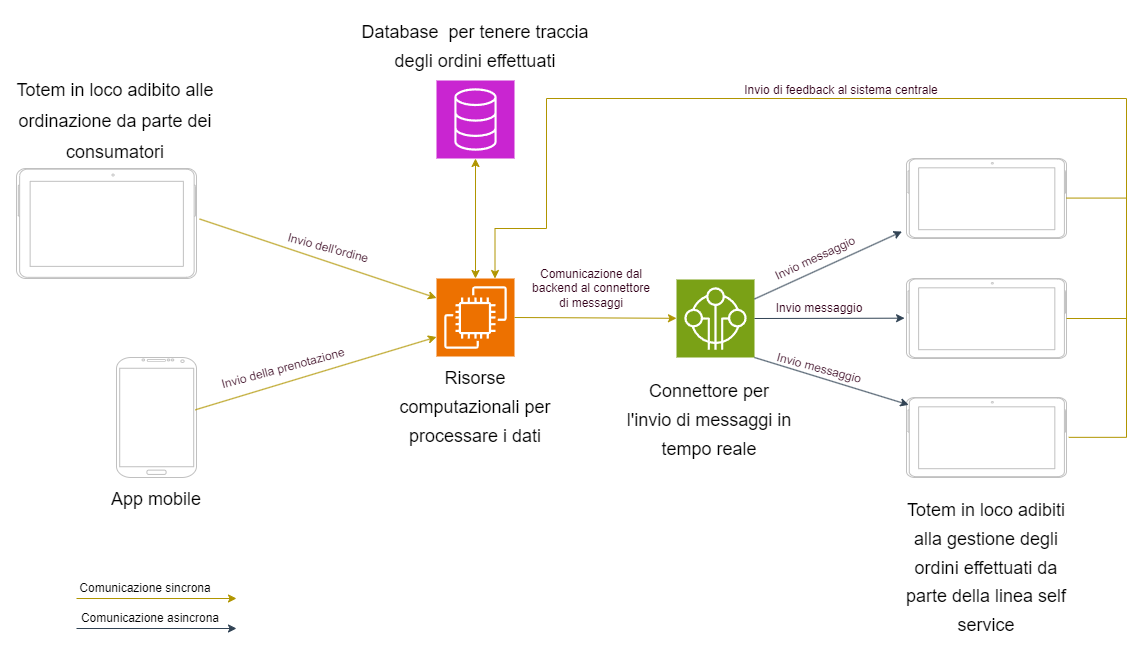
\includegraphics[scale=0.40]{architettura}
\centering
\end{figure}

In riferimento alla figura 2.1, possiamo suddividere l'architettura in 4 tipologie di elementi:
\begin{itemize}
	\item \textbf{Interfacce per la creazione di ordini}: nel nostro caso tramite totem in loco e app mobile. Sia l'app che il totem possono essere realizzati con Flutter, un innovativo framework per lo sviluppo di app cross-platform che funziona per iOS, Android, Linux, Windows e Web. La scelta di questo framework rappresenta un grande
				 vantaggio competitivo e strategico, in quanto:
				 \begin{itemize}
				 	\item garantisce correttezza e "feature-parity" tra le varie piattaforme, in quanto realizzate tutte a partire da un unico codice sorgente
				 	\item consente di iniziare lo sviluppo con un team di persone limitato, in quanto è possibile selezionare solamente figure con skills omogenee
				 	\item al momento è il framework più popolare del mercato per la creazione di app mobili, avendo superato React Native. Rappresenta quindi una scelta solida su cui investire anche a livello di management aziendale \cite{flutterreact}
				    \item avendo la possibilità di creare interfacce anche per iOS e Android, ci consente di raggiungere un bacino di utenti molto più ampio rispetto ad una pagina web
				    	  navigabile da pc fisso o portatile \cite{hardwaremob}
				 \end{itemize}
				 
	\item \textbf{Risorse per la computazione dei dati}: nel nostro progetto abbiamo necessità di avere uno o più copie dell'applicativo che gestisce tutte le operazioni
				 di logica delle code e di archiviazione dei dati in esecuzione contemporaneamente, al fine di poter sostenere la crescita orizzontale del sistema in base al numero di ubicazioni attive. In particolare, possiamo suddividere le risorse in due componenti:
				 \begin{itemize}
				 	\item \textbf{Un database SQL}: in particolar modo PostgreSQL, facilmente scalabile, ACID-compliant ed open source. La scelta di un database SQL rispetto ad
				 				 un database NoSQL è stata influenzata dall'incapacità dei database NoSQL di creare vincoli UNIQUE, cosa che a noi interessa
				 				 al fine di evitare inserimenti doppi di individui in coda e semplificare i problemi di concorrenza
				 	\item \textbf{Un applicativo}: lo stack di questo applicativo varia dalle necessità dell'azienda, ma soprattutto dalle skills tecnologiche già presenti
				 				 all'interno dell'azienda. Un linguaggio che sicuramente può soddisfare le esigenze del nostro applicativo è GoLang:
				 				 \begin{itemize}
				 				 	\item ogni programma scritto in go è facilmente containerizzabile e deployabile su qualsiasi infrastruttura moderna come Kubernetes
				 				 	\item ll linguaggio è semplice da apprendere e gestire con poche ambiguità, perfetto sia per grandi aziende che per startup
				 				 	\item l'ecosistema per la scrittura di applicativi web concorrenti è molto vasto, avendo una user-base che sviluppa principalmente 
				 				 		  applicativi web o applicativi di rete
				 				 	\item la concorrenza è un cittadino di prima classe tramite "Goroutines" e "Channels"
				 				 \end{itemize}
				 				 L'applicativo dovrà esporre una serie di chiamate HTTP per permettere di effettuare tutte le operazioni necessarie,
				 				 e dovrà poter comunicare direttamente con il connettore di invio messaggi e il database sql. L'applicativo è state-less, ovvero non tiene nulla nella sua memoria, e processa i dati singolarmente per ogni richiesta. Questa scelta è fatta per permettere l'aggiunta / distruzione di istanze on-the-fly tramite
				 				 Kubernetes senza doversi preoccupare di sincronizzare le varie istanze tra di loro.
				 \end{itemize}
	
	\item \textbf{Connettore per l'invio di messaggi in tempo reale}: questo componente ha il compito di creare degli specifici canali d'ascolto chiamati "topic",
				 a cui i client possono connettersi ed ascoltare i messaggi inviati nei canali da loro scelti e a loro volta scrivere all'interno dei canali. Questa funzionalità è erogata tramite il protocollo di comunicazione MQTT utilizzando il modello Pub/Sub. Nel nostro caso, MQTT mette a disposizione dei canali al cui interno vengono inviati
				 dei messaggi JSON codificati in base64. Il nome di ogni canale ha la seguente struttura: \textbf{id-univoco-cliente/devices/id-univoco-device}.
				 Ogni device fisico si mette in ascolto sul canale che corrisponde al suo id, così da ricevere solamente i messaggi a lui riservati. In caso di messaggi "globali"
				 per tutti i device collegati ad una particolare coda, è possibile utilizzare il canale con la seguente struttura: \textbf{id-univoco-cliente/queues/id-univoco-coda}.
				 Il protocollo MQTT ci garantisce l'invio dei messaggi al meglio di uno, non escludendo quindi la possibilità di ricevere messaggi duplicati. Sarà nostro compito
				 capire come ignorare eventuali messaggi duplicati. Nella nostra configurazione, i dispositivi fisici fungono solamente da subscribers, e l'unico publisher è 
				 il sistema centrale, che invierà messaggi al connettore tramite una chiamata HTTP dedicata che funge da ingest dei messaggi. 
				 Si è scelto di fare affidamento ad AWS IoT, un servizio cloud completamente gestito e scalabile fino a 100 milioni
				 di messaggi al secondo e oltre 10 milioni di dispositivi connessi contemporaneamente.
				 
	\item \textbf{Interfacce per la gestione dei flussi}: analogo al caso delle interfacce per gli ordini, la scelta più adatta rimane Flutter.
	
\end{itemize}

\subsection{La vita di un flusso di coda}
Procediamo ora ad illustrare come viene creato e completato un flusso di coda a partire da un utente che effettua un ordine in loco:
\begin{enumerate}
	\item L'utente completa l'acquisto sul totem delle ordinazioni
	\item Il totem invia una richiesta HTTP al sistema centrale per verificare la validità dell'ordine
	\item Supponendo che la verifica sia andata a buon fine, il sistema centrale procede attraverso la sezione critica di assegnare un numero univoco all'ordine
		  e una volta determinato lo restituisce al totem in risposta alla chiamata HTTP. Infine il totem stampa all'utente il codice ricevuto.
	\item Una volta determinato il codice, contemporaneamente alla risposta per il totem il sistema centrale procede a determinare quali dispositivi vanno avvisati dell'arrivo dell'utente, e successivamente invia una richiesta HTTP al punto di ingest del componente MQTT, fornendo il messaggio da inviare e i canali destinatari. Nel nostro caso, ci troviamo alla creazione del flusso e di conseguenza questo messaggio verrà recapitato al dispositivo assegnato alla postazione dei primi piatti.
	\item Una volta che il messaggio è stato ricevuto, viene inserito nella coda locale all'interno del dispositivo ed avanzerà man mano al comando dell'operatore.
	\item Alla richiesta di avanzamento da parte dell'operatore del nostro messaggio, il dispositivo invia una chiamata HTTP al sistema centrale, chiedendo l'avanzamento del flusso
		  corrente al dispositivo successivo. Il sistema centrale computa il ricevente successivo, e procede a recapitare il messaggio sempre tramite il componente MQTT.
	\item Il ciclo si ripete fino a quando, arrivati all'ultimo dispositivo fisico, il sistema determina che il flusso è terminato, e procede al suo completamento,
		  dismettendo i messaggi inerenti al flusso. 
\end{enumerate}

Dall'illustrazione possiamo notare come il corretto funzionamento dell'intero sistema dipenda da un perfetta armonia tutti gli elementi coinvolti. E' per tanto molto importante affrontare seriamente tutte le possibili criticità che possono presentarsi.

\subsection{Analisi criticità: Ridondanza del sistema centrale}

Come descritto in precedenza, avendo delegato il compito al sistema centrale di gestire le logiche di ordine e avanzamento, è necessario che questo sia sempre operativo
e raggiungibile da qualsiasi parte del mondo. Per questo motivo, appoggiarsi a un provider cloud con servizi gestiti è sicuramente una scelta farevole. I provider cloud mascherano
la complessità di gestire una infrastruttura ridondata e si occupano loro di garantire percentuali di uptime annuali molto alte, fino a 99.995\%, ovvero meno di 30 minuti di disservizio l'anno. Non è però sufficiente scegliere una infrastruttura sicura, ma è necessario progettare anche l'intera architettura per resistere agli errori imprevisti, gestire la scalabilità durante i picchi, e saper recuperare le informazioni in caso di distruzione del servizio. Uno strumento adatto a questo compito è Kubernetes, un framework nato per semplificare lo scaling di applicazioni in maniera uniforme, sfruttando la tecnologia dei container linux. Possiamo quindi utilizzare:
\begin{itemize}
	\item \textbf{AWS EC2} per le risorse computazionali pure
	\item \textbf{AWS EKS} per la gestione delle risorse tramite Kubernetes
	\item \textbf{AWS RDS} per un database sql postgres replicato
	\item \textbf{AWS IOT} come connettore MQTT distribuito
	\item \textbf{AWS S3} per salvare tutti i backup dei dati ad intervalli regolari (es: ogni 6 ore)
\end{itemize}

\subsection{Analisi criticità: Determinare l'ordine dei dispositivi nella coda virtuale}

Uno dei primi problemi da risolvere è capire come strutturare una anagrafica per salvare l'ordine dei dispositivi all'interno di una coda prevenendo doppioni.
Questo problema può essere risolto sfruttando una delle caratteristiche dei database SQL, ovvero il vincolo \textbf{UNIQUE}.
La nostra tabella dati può essere strutturata nel seguente modo:

\begin{center}
    \begin{tabular}{ | l | l | p{3cm} | p{3cm} |}
    \hline
    Nome colonna & Tipologia & Argomenti & Descrizione \\ \hline
    id & INT(11) UNSIGNED & NOT NULL PRIMARY KEY & Chiave primaria della riga di associazione. \\ \hline
    dispositivo\_fisico\_id & INT(11) UNSIGNED & NOT NULL & ID del dispositivo da associare alla coda. \\ \hline
    coda\_id & INT(11) UNSIGNED & NOT NULL & ID della coda a cui associare il dispositivo. \\ \hline
    dispositivo\_ordine & INT(2) UNSIGNED & NOT NULL & Ordine virtuale del dispositivo a partire da 1. \\ \hline
    \end{tabular}
\end{center}

Questa struttura dati ci consente di associare qualsiasi dispositivo fisico a qualsiasi coda ed in qualsiasi ordine. Noi vogliamo associare un dispositivo solamente una volta ad una coda, e vogliamo assicurarci che per essa non ci siano mai due dispositivi con lo stesso ordine. Per farlo, possiamo utilizzare due vincoli UNIQUE:
\begin{itemize}
	\item \textbf{UNIQUE(dispositivo\_fisico\_id, coda\_id)}: al fine di tenere attivo il principio che un dispositivo fisico può essere collegato solamente ad una coda contemporaneamente
	\item \textbf{UNIQUE(dispositivo\_ordine, coda\_id)}: al fine di tenere attivo il principio che non possono esistere più dispositivi nella stessa coda con lo stesso ordine
\end{itemize}

\subsection{Analisi criticità: ottenimento del numero in coda}

Il numero in coda è il modo con cui il sistema comunica agli utenti, all'interno del refettorio, la propria posizione in coda. Determinarlo in un ambiente corrente non è banale, in quanto vi è la possibilità di creare dei numeri duplicati se non gestiti correttamente. Per aggirare questa criticità, possiamo fare affidamento alle funzionalità offerte dal database SQL, utilizzando una transazione atomica combinata ad un lock sulla tabella in scrittura e lettura.

\begin{algorithm}
\caption{gestione ottenimento numero di coda}
\begin{algorithmic}[1]
\State $tentativi \gets 5$
\State $nuovoNumero \gets -1$
\While{$tentativi \ge 0$}
\State acquisisci lock sulla tabella con timeout di 100ms
\If{lock acquisito}
\State leggi ultimo numero inserito nella tabella
\State $nuovoNumero \gets ultimoNumero + 1$
\State salva a database il flusso con una transazione atomica
\State rilascia il lock
\State break
\Else
\State $tentativi \gets tentativi - 1$
\EndIf
\EndWhile
\If{$nuovoNumero$ == -1}
\State throw errore inserimento fallito
\EndIf
\end{algorithmic}
\end{algorithm}

Questo algoritmo garantisce di non avere deadlock perchè una risorsa non viene mai tenuta per un tempo indefinito. Allo stesso tempo, si assicura che durante la fase critica concessa dal lock il dato su cui stiamo lavorando sia sempre integro.

\subsection{Analisi criticità: gestire l'invio di messaggi relativi ai cambiamenti nella coda}

L'invio dei messaggi inerenti ai cambiamenti della coda necessità delle seguenti proprietà:

\begin{itemize}
	\item \textbf{Riproducibilità}: il dispositivo fisico che riceve i messaggi deve poter richiedere nuovamente l'invio del messaggio in qualsiasi momento
	\item \textbf{Univocità}: all'interno del sistema centrale, deve esistere un identificatore univoco che descrive ogni messaggio, così che i consumer possano distinguere eventuali messaggi duplicati
\end{itemize}

Iniziamo affrontando il problema dell'univocità. Questo può essere facilmente affrontato facendo ancora una volta riferimento alle qualità offerte dal database. Ogni riga di flusso attivo salvata a database riceve un ID univoco che identifica singolarmente quella riga all'interno della tabella dati. Considerato che nella tabella sono presenti tutti i flussi gestiti dal sistema centrale, possiamo affermare che possediamo un modo univoco per distinguere ogni riga di flusso attivo.
\newline
Abbiamo ora bisogno di un metodo per capire se un flusso è stato modificato dall'ultima volta che è stato ricevuto. Confrontare ogni parametro all'interno del flusso non è scalabile e risulta complicato, poichè potrebbero co-esistere versioni di schema database di flussi diversi. Possiamo però introdurre una colonna denominata \textbf{last\_update} in cui salvare l'ultima volta che la riga di flusso è stata modificata, valorizzando la colonna con uno unix timestamp misurato in microsecondi.
\newline
Possiamo ora combinare l'id univoco e il timestamp formando una chiave d'identificazione composta \textbf{ID\_UNIVOCO.LAST\_UPDATE} con:
\begin{itemize}
	\item \textbf{Una parte fissa} che non cambia mai e identifica univocamente il flusso all'interno del sistema
	\item \textbf{Una parte dinamica} che può cambiare a seconda di quante volte viene modificato il flusso, consentendo di rilevare i cambiamenti
\end{itemize}
Passiamo ora a risolvere il problema della riproducibilità. Come descritto precedentemente, in qualsiasi momento possono verificarsi dei casi per cui il dispositivo può avere necessità di effettuare una sincronizzazione. E' quindi necessario sviluppare un endpoint dedicato a ritornare i flussi attivi di quel particolare dispositivo all'interno del sistema centrale per poter completare questa operazione. Possiamo identificare questa procedura come "operazione di sincronizzazione". \textbf{Il sistema centrale viene sempre considerato come la fonte di verità in caso di incongruenze}. Per scrivere e leggere all'interno della coda locale al dispositivo, il software installato al suo interno utilizza un lock per gestire la concorrenza tra avanzamento automatico, avanzamento da parte dell'operatore, ricezione di messaggi asincroni e sincronizzazione con il sistema centrale.

\begin{algorithm}
\caption{gestione della sincronizzazione interna al dispositivo}
\begin{algorithmic}[1]
\State acquisisci lock lettura e scrittura sulla coda locale per un massimo di 5 secondi
\If{lock non acquisito}
\State throw eccezione impossibile completare sincronizzazione
\EndIf
\State effettua la chiamata HTTP al sistema centrale per ottenere tutti i flussi attivi
\If{chiamata fallita}
	\State rilascia lock lettura e scrittura
	\State throw eccezione impossibile completare sincronizzazione
\EndIf
\ForAll{flussi ottenuti dal sistema}
	\If{flusso non presente in coda locale}
		\State aggiungi il flusso alla coda locale
	\ElsIf{flusso presente e con chiave composta diversa}
		\State sostituisci il flusso nella coda locale con il flusso aggiornato
	\EndIf
\EndFor
\State esegui intersezione tra la coda locale e la lista di flussi ottenuta per rimuovere eventuali flussi non sincronizzati
\State rilascia il lock in lettura
\State aggiorna la UI del dispositivo
\State rilascia il lock in scrittura
\end{algorithmic}
\end{algorithm}

\section{Considerazioni finali}

Abbiamo quindi visto come progettare e avviare un sistema per gestire un refettorio aziendale. Vediamo ora alcune considerazioni finali sul progetto:

\begin{itemize}
\item E' consigliabile effettuare molteplici test di carico del sistema, riproducendo l'entrata e l'uscita di molti utenti contemporaneamente, l'invio di ordini e prenotazioni simultaneamente e l'aggiunta di parecchi dispositivi operatore nella stessa ubicazione, misurando per simulazione le tempistiche di ogni componente all'interno dell'architettura. Questi "stress test" saranno specialmente utili per calibrare le delicate tempistiche dei lock che gestiscono le sezioni critiche.
\item Budget permettendo, è raccomandabile l'utilizzo di dispositivi fisici con sistema operativo Android, al fine di poter usufruire dei google play services e degli aggiornamenti delle app tramite play store o MDM interno.
\item Si sconsiglia vivamente l'utilizzo di sistemi operativi Windows per l'applicativo centrale, sia per le performance ridotte dei container rispetto ad un ambiente Linux, sia per i costi aggiuntivi di acquisto delle licenze.
\item Per identificare degli utenti aziendali che effettuano l'accesso alla mensa, si suggerisce l'uso di rilevatori di badge magnetici o rilevatori ottici per la scansione di tesserini. Questo tipo di rilevatori è tendenzialmente molto veloce nella lettura, divenendo un candidato ideale per un ambiente ad alta concentrazione di utenti.

\end{itemize}

\chapter{Terminologie}\label{chap:terminologie}

\begin{itemize}
	\item \textbf{FAANG}: Facebook, Apple, Amazon, Netflix, Google
	\item \textbf{AGID}: Agenzia per l'Italia Digitale
	\item \textbf{ACID}: Atomicity, Consistency, Isolation, e Durability
	\item \textbf{Go-routines}: Funzioni one-shot che vengono eseguite in thread "leggeri" grazie ai costi ridotti per la loro creazione rispetto ai thread tradizionali
	\item \textbf{Channels}: Strumento che consente lo scambio di messaggi tra go-routine diverse senza la necessità di avere memoria condivisa
	\item \textbf{MQTT}: Message Queuing Telemetry Transport, protocollo ISO che funziona su TCP/IP
	\item \textbf{Kubernetes}: Sistema open source di orchestrazione e gestione di container distribuiti su macchine differenti
	\item \textbf{JSON}: JavaScript Object Notation, formato per lo scambio dati basato sul linguaggio di programmazione JavaScript
	\item \textbf{AWS}: Amazon Web Services, azienda leader nel settore cloud computing di proprietà di Amazon
	\item \textbf{MDM}: Mobile Device Management, piattaforma che permette la gestione di tutti gli aspetti di un dispositivo remoto
	\item \textbf{Pub/Sub}: Publisher/Subscriber, design pattern utilizzato per la comunicazione asincrona fra diversi processi, oggetti o agenti.
\end{itemize}

\chapter{Dedica}\label{chap:dedica}

Ci tengo a sottolineare che tutte le persone in questo elenco hanno avuto un ruolo importante all'interno di questo mio percorso universitario, e che l'ordine in cui sono scritti non simboleggia la loro importanza. Detto questo, voglio ringraziare:

\begin{itemize}
	\item \textbf{I miei genitori} che nonostante tutte le mie scelte sbagliate, le mie mancanze di rispetto nei loro confronti, il mio ritardo nel completare l'università e il mio carattere non sempre aperto a critiche, mi hanno sempre stimolato a crescere sia caratterialmente che professionalmente, fin da bambino mi hanno sempre valorizzato mettendomi al primo posto in tutte le loro decisioni e mi hanno riportato più volte sulla giusta strada anche quando il percorso universitario era ad un passo dal terminare prematuramente, senza mai farmi sentire in difetto nei loro confronti e senza mai pretendere un ringraziamento
	\item \textbf{La mia fidanzata Simona} che fin dai primi momenti assieme mi ha sempre sostenuto e spronato a fare di meglio, ed in questi quattro anni pieni di alti e bassi è sempre stata senza indugio il punto fermo a cui fare riferimento per ogni mio problema
	\item \textbf{I miei compagni di studio} che hanno sopportato tutte le mie lamentele nei confronti delle materie universitarie (e fidatevi, erano tante). Ad alcuni di loro devo un ringraziamento speciale perchè attraverso la loro pazienza nello spiegarmi gli argomenti decine di volte, sono riusciti a farli entrare in questa testa dura
	\item \textbf{La squadra di RistoCloud} ovvero l'azienda che in questi anni mi ha permesso di maturare sia professionalmente fornendomi tutti gli strumenti necessari per crescere e apprendere nuove abilità tecniche sia umanamente insegnandomi come si comunica e come ci si rapporta in gruppo di persone. Mi hanno inoltre dato la possibilità di auto sostenere il mio percorso universitario senza gravare sulle spalle dei miei genitori, ma soprattutto mi hanno fatto vivere dei momenti indimenticabili tra progetti falliti, progetti riusciti, celebrazioni di gruppo e riti inusuali come quello delle paste al mercoledì. Nonostante la mia poca presenza di persona, ad ogni mio salire in ufficio sono sempre stato accolto con calore da quelli che oggi posso definire amici oltreché colleghi e di questo ve ne sono grato.
\end{itemize}

\begin{thebibliography}{9}
	\bibitem{cornell} Susan Kelley. \textsl{Groups that eat together perform better together}. Cornell University, 2015
	\bibitem{rristorazione} Fipe. \textsl{Ristorazione - Rapporto annuale 2023}. Confcommercio, 2023
	\bibitem{hardwaremob} Statista. \textsl{Market share of desktop, mobile, tablet, and console devices in Italy from 2016 to 2022}. Statista, 2023
	\bibitem{flutterreact} Flatirons. \textsl{Popularity of Flutter vs. React Native in 2024}. Flatirons, 2024
\end{thebibliography}

\end{document}
